\subsection{Regularization and Variable Selection}

We now apply three of the previously discussed priors to linear and logistic models using synthetic data (consisting of training and test sets) under two settings:

\begin{itemize}
    \item \textbf{Scenario A}: A well-behaved setting without collinearity to examine shrinkage:
    \begin{equation*}
        \begin{aligned}
            &n = 150,\; n_{train} = 100,\;n_{test} = 50, \\
            &\btheta = (2, 1.5, 0, 0, 0), \\
            &\bX \sim \Ncal(\bnull, \bI), \\
            &\text{linear: } \by \mid \btheta \sim \Ncal(\bX \btheta,\bI), \quad \text{logistic: } \by \mid \btheta \sim \text{Ber}(\sigma(\bX \btheta)).
        \end{aligned}
    \end{equation*}
    \item \textbf{Scenario B}: A low-information setting where $n \approx p$ with collinearity between informative and non-informative covariates:
    \begin{equation*}
        \begin{aligned}
            &n = 150,\; n_{train} = 30,\;n_{test} = 120, \\
            &\btheta = (2, 1.5, 0, \overset{26\; \text{times}}{\dots}, 0), \\
            &\bX \sim \Ncal(\bnull, \Sd), \quad \Sd =
                    \begin{pmatrix}
                    1 &        &         &        &        \\
                        & \!\!S_3\!\! &        & 0      &        \\
                        &        & I_{26} &        &        \\
                        & 0      &        &        &        \\
                    \end{pmatrix},
                    \qquad
                    S_3 = 
                    \begin{pmatrix}
                    1   & 0.8 & 0.8\\
                    0.8 & 1   & 0.8\\
                    0.8 & 0.8 & 1
                    \end{pmatrix},\\
            &\text{linear: } \by \mid \btheta \sim \Ncal(\bX \btheta, \bI), \quad \text{logistic: } \by \mid \btheta \sim \text{Ber}(\sigma(\bX \btheta)).
        \end{aligned}
    \end{equation*}
\end{itemize}

For each scenario, we fit three linear and three logistic regression models using the following priors: A flat prior as a benchmark, using the conjugate setting described in \autoref{eq:flat-prior} with the R-package \texttt{brms} \citep{brms_2017}.\footnote{To obtain a virtually flat prior, the Gaussian prior variance was set to $10^6$ and the Gamma prior parameters were set to $a = 0.001, b=0.001$, which results in an uninformative prior.} 
We fit a ridge prior (see \autoref{eq:ridge}) and a LASSO prior (see \autoref{eq:lasso}) via the \texttt{bayesreg} package \citep{makalic_bayesreg_2016} with automated optimization of the regularization parameters $\tau^2$ and $\lambda^2$.
For all models, we ran MCMC with 20,000 iterations, a 1,000 burn-in, and a thinning interval of 10.\\

Our evaluation focused on two aspects:
Firstly, \textit{variable selection accuracy}, i.e.\@ the number of correctly identified influential covariates (Hits) and falsely as influential declared covariates (FP).
Although ridge and LASSO shrink coefficients, they do not perform variable selection by themselves.
Thus, we used Bayesian credibility intervals as a criterion to decide whether a parameter is credibly nonzero as described in \citet{van_erp_shrinkage_2019}.
Secondly, \textit{predictive accuracy}.
This was measured on the test set by the mean log posterior predictive density (MLPPD) proposed by \citet{gelman_understanding_2013}.
Since the log-likelihood is a proper scoring rule, it is well-suited to evaluate Bayesian models.\\

\begin{table}[ht]
    \small
    \centering
    \begin{tabular}{@{} ll  rrr   rrr @{}}
        \toprule
        Model & Prior 
            & \multicolumn{3}{c}{Scenario A} 
            & \multicolumn{3}{c}{Scenario B} \\
        \cmidrule(lr){3-5} \cmidrule(lr){6-8}
                &      
            & Hits (of 2) & FP (of 3)  & MLPPD      
            & Hits (of 2) & FP (of 28) & MLPPD     \\
        \midrule
        %---- Linear block
        Linear & flat   & 2 &  0 & -1.425  
        & 2 &  1 &   -1.605     \\
        Linear & LASSO  & 2 &  0 & -1.424  
                & 2 &  0 &   -1.464     \\
        Linear & ridge  & 2 &  0 & -1.427  
                & 2 &  0 &   -1.575     \\
        \specialrule{1.5pt}{0pt}{0pt}
        %---- Logit block
        Logit  & flat   & 2 &  1 & -0.390  
        & 0 & 21 &   $-\infty$  \\
        Logit  & LASSO  & 1 &  0 & -0.463  
        & 1 &  0 &   -0.485     \\
        Logit  & ridge  & 1 &  0 & -0.455  
        & 1 &  0 &   -0.493     \\
        \bottomrule
    \end{tabular}
    \caption{Evaluation metrics of Bayesian linear and logistic regression, each with a flat, ridge, and LASSO prior, under Scenarios A and B.
    }
    \label{tab:reg_AB}
\end{table}

\autoref{tab:reg_AB} shows numerical results, while \autoref{fig:reg-params} visualizes parameter estimates and uncertainty.
For linear regression, all priors correctly identified the influential variables and produced few or no false positives.
The effect of regularization is more pronounced in logistic regression: in both scenarios, the regularized models (LASSO and ridge) declared fewer coefficients as influential and reduced false positives.
In the low-information Scenario B, regularization priors improved both variable selection and predictive accuracy (MLPPD). Except under the flat prior, Bayesian logistic regression achieved slightly better predictive performance than linear regression, although differences in MLPPD between priors were minimal. Conversely, linear models provided more accurate estimates with narrower CIs than logistic models.
In Scenario B, the uncertainty of the unregularized logistic model becomes especially evident, highlighting the importance of regularization in high-dimensional, low-information settings.

\begin{figure}[htbp]
    \centering
    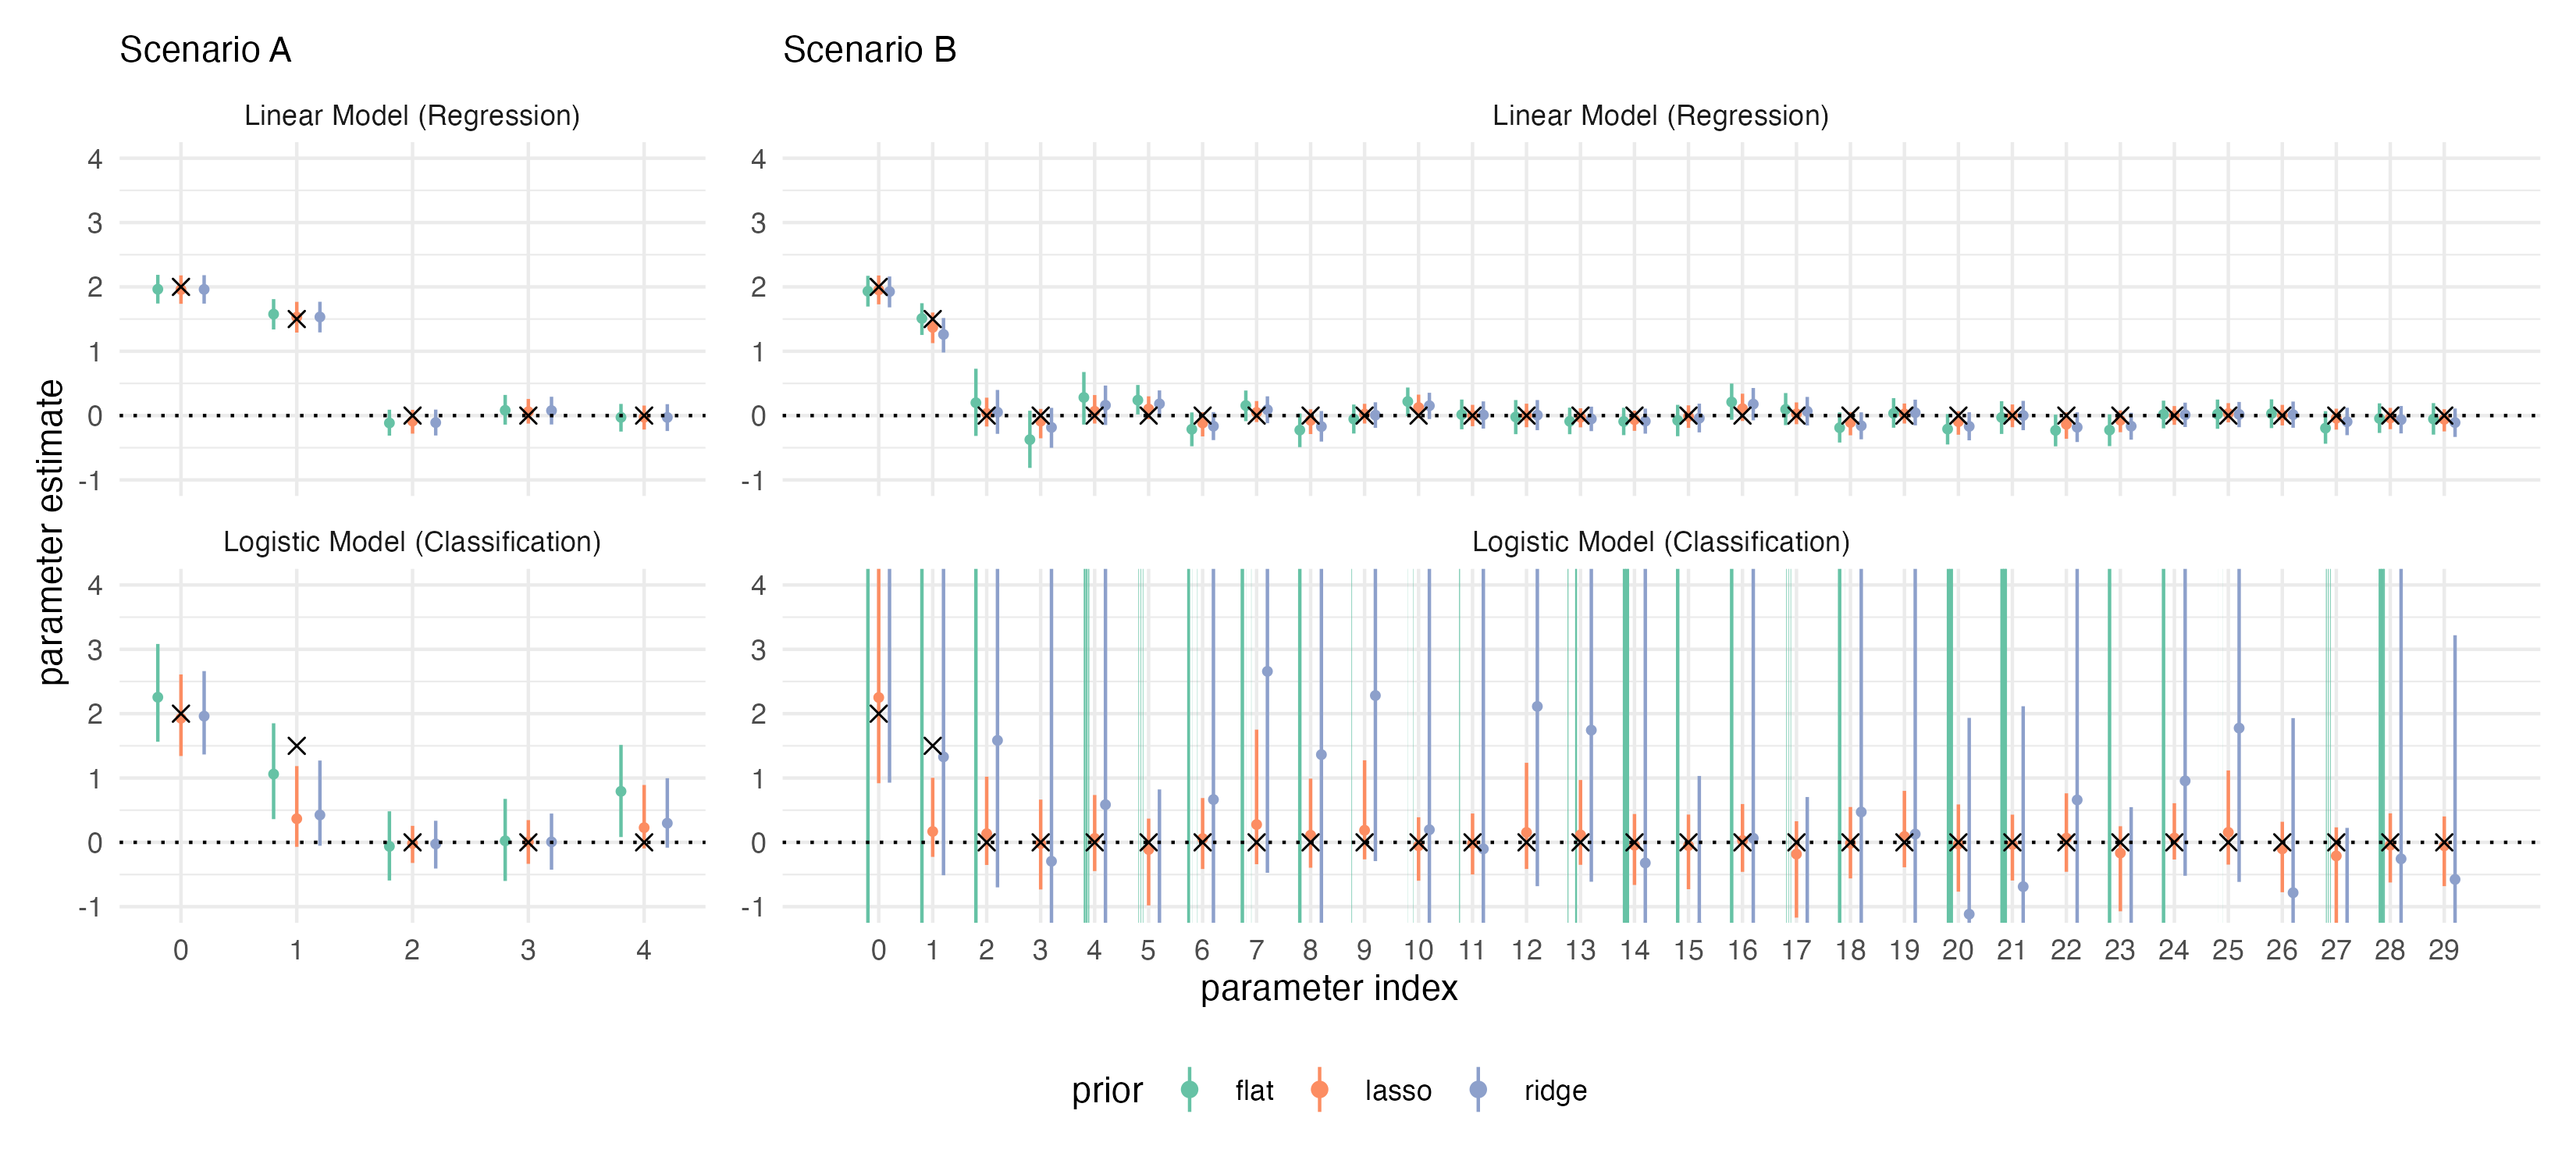
\includegraphics[width=\linewidth]{../figures/reg_all.png}
    \caption{Estimated model parameters with 95\% credibility intervals (CI).
    True parameter values are black crosses.
    }
    \label{fig:reg-params}
\end{figure}

\subsection{Performance of Approximate Inference Algorithms}

In this second experiment, we compared LA and Metropolis-Hastings MCMC in Bayesian linear and logistic regression.\\

We generate 1,000 synthetic data sets with $n=100$:
\begin{equation*}
    \begin{aligned}
        &\bX \sim \Ncal(\bnull, \bI), \quad \btheta = (-0.5, 2, 1)\\
        &\text{linear: } \by \mid \btheta \sim \Ncal(\bX \btheta, \bI),\quad \text{logistic: } \by \mid \btheta \sim \text{Ber}(\sigma(\bX \btheta))
    \end{aligned}
\end{equation*}

Each data set was used to fit one linear and one logistic model, using both inference approaches.
We assumed $\btheta \sim \Ncal(0, 10 \cdot \bI)$ and fixed residual variance  at $\ssd = 10$.
For LA, we used \texttt{r-INLA} \citep[][\url{ www.r-inla.org}]{rue_approximate_2009} with settings to default from INLA to simple LA.
For MCMC, we used the \texttt{MCMCglmm} package \citep{MCMCglmm_2010} with settings specifically to use Metropolis-Hastings, a relatively small sample size of 5,000, a burn-in period of 500, and a thinning interval of 10.
For each method, we recorded CPU runtime, posterior means, and posterior standard deviations of the estimated parameters.\\

\begin{figure}[htbp]
    \centering
    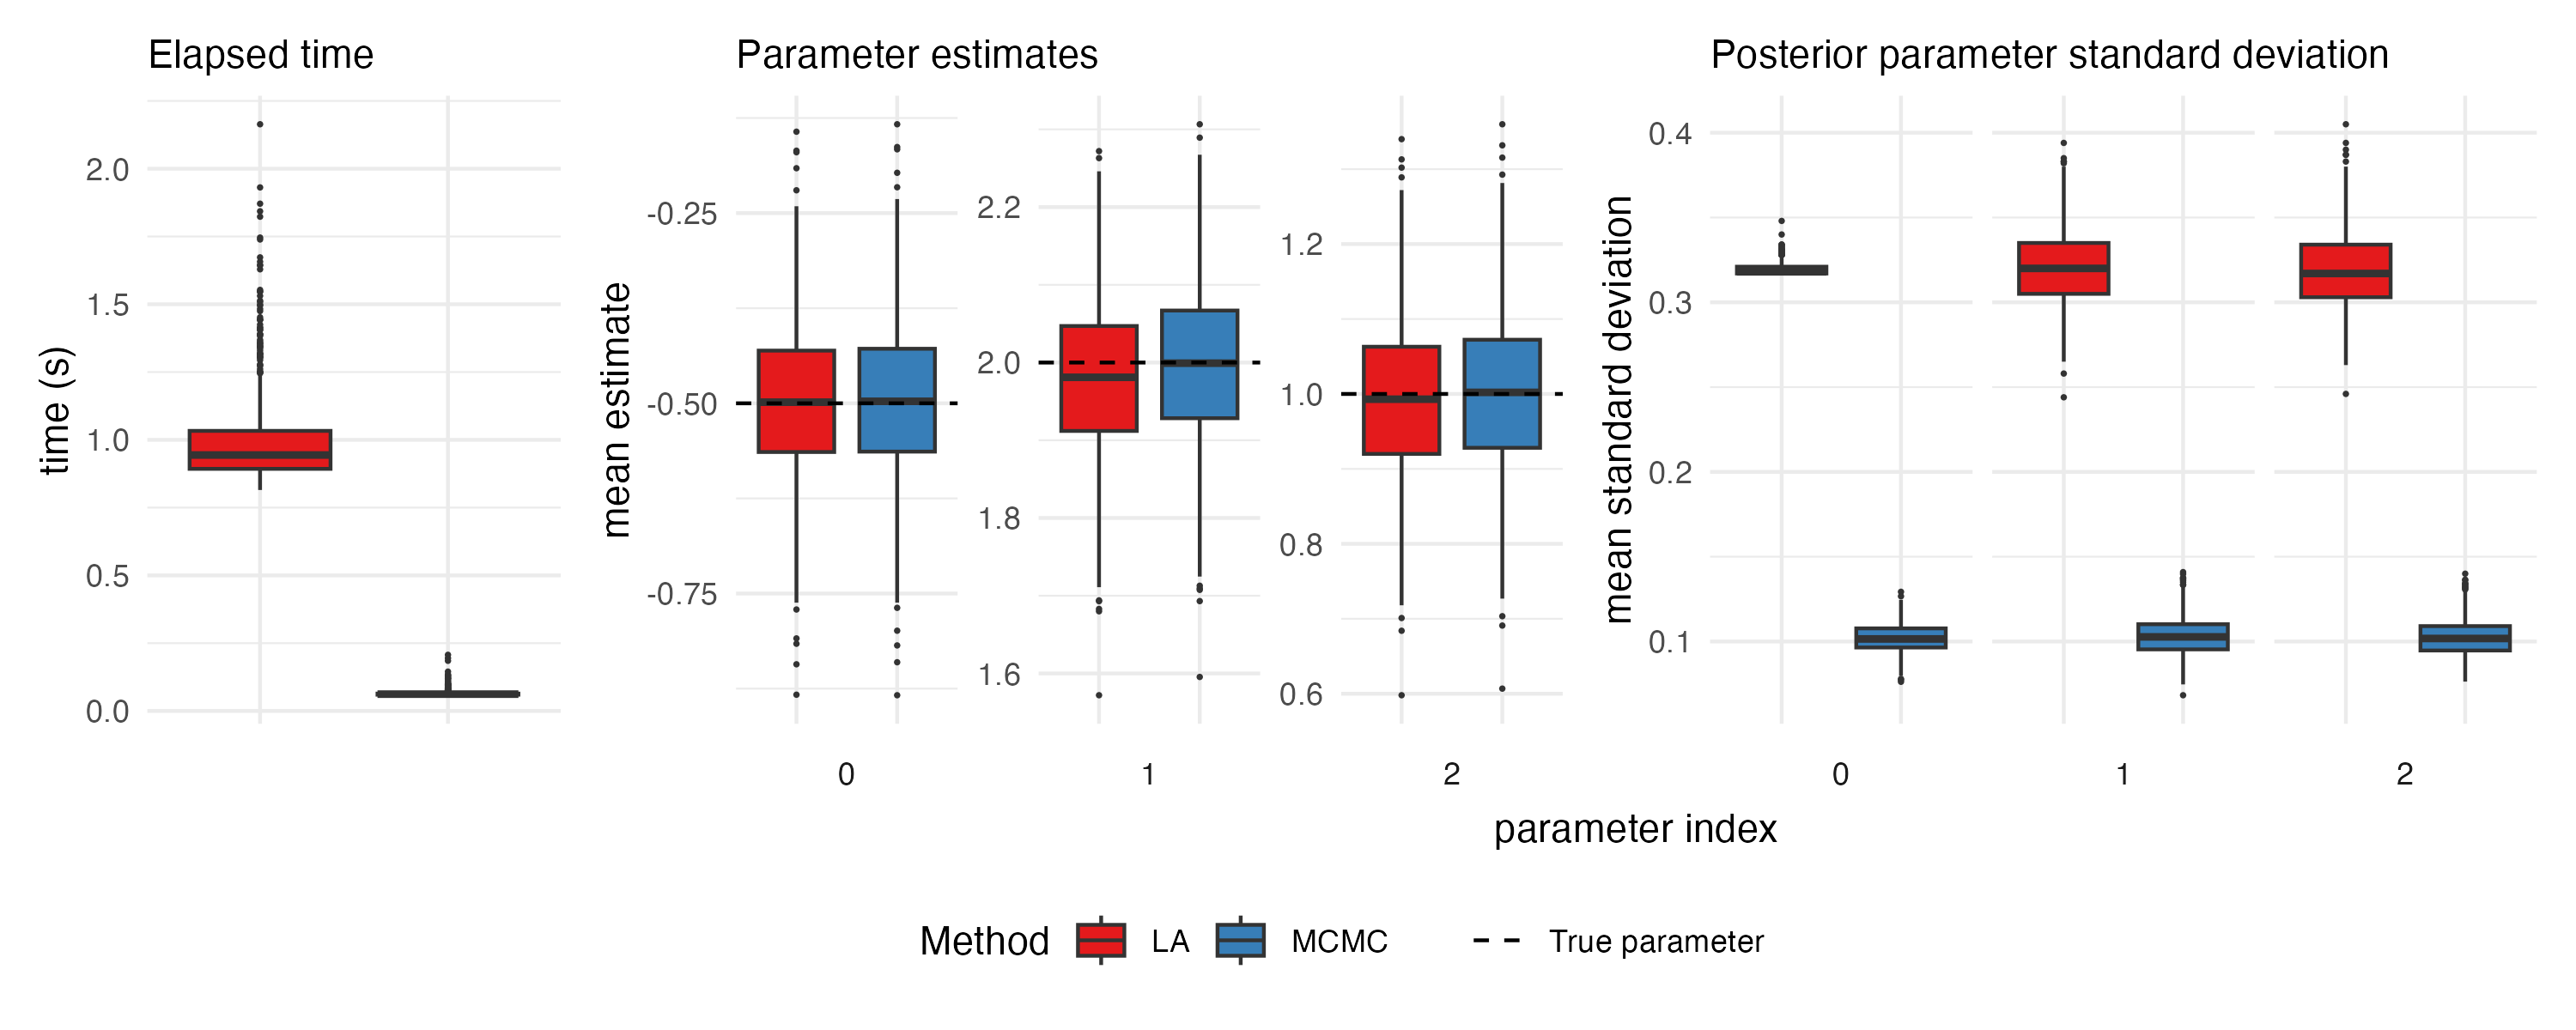
\includegraphics[width=\linewidth]{../figures/approx_regr.png}
    \caption{
    Bayesian \textbf{linear} regression: Comparison of LA (red) and MCMC (blue) across 1,000 simulations.
    MCMC is faster in this case.
    Both methods estimate the parameters accurately, though LA yields higher posterior uncertainty.
    }
    \label{fig:approx-regr}
\end{figure}

\begin{figure}[htbp]
    \centering
    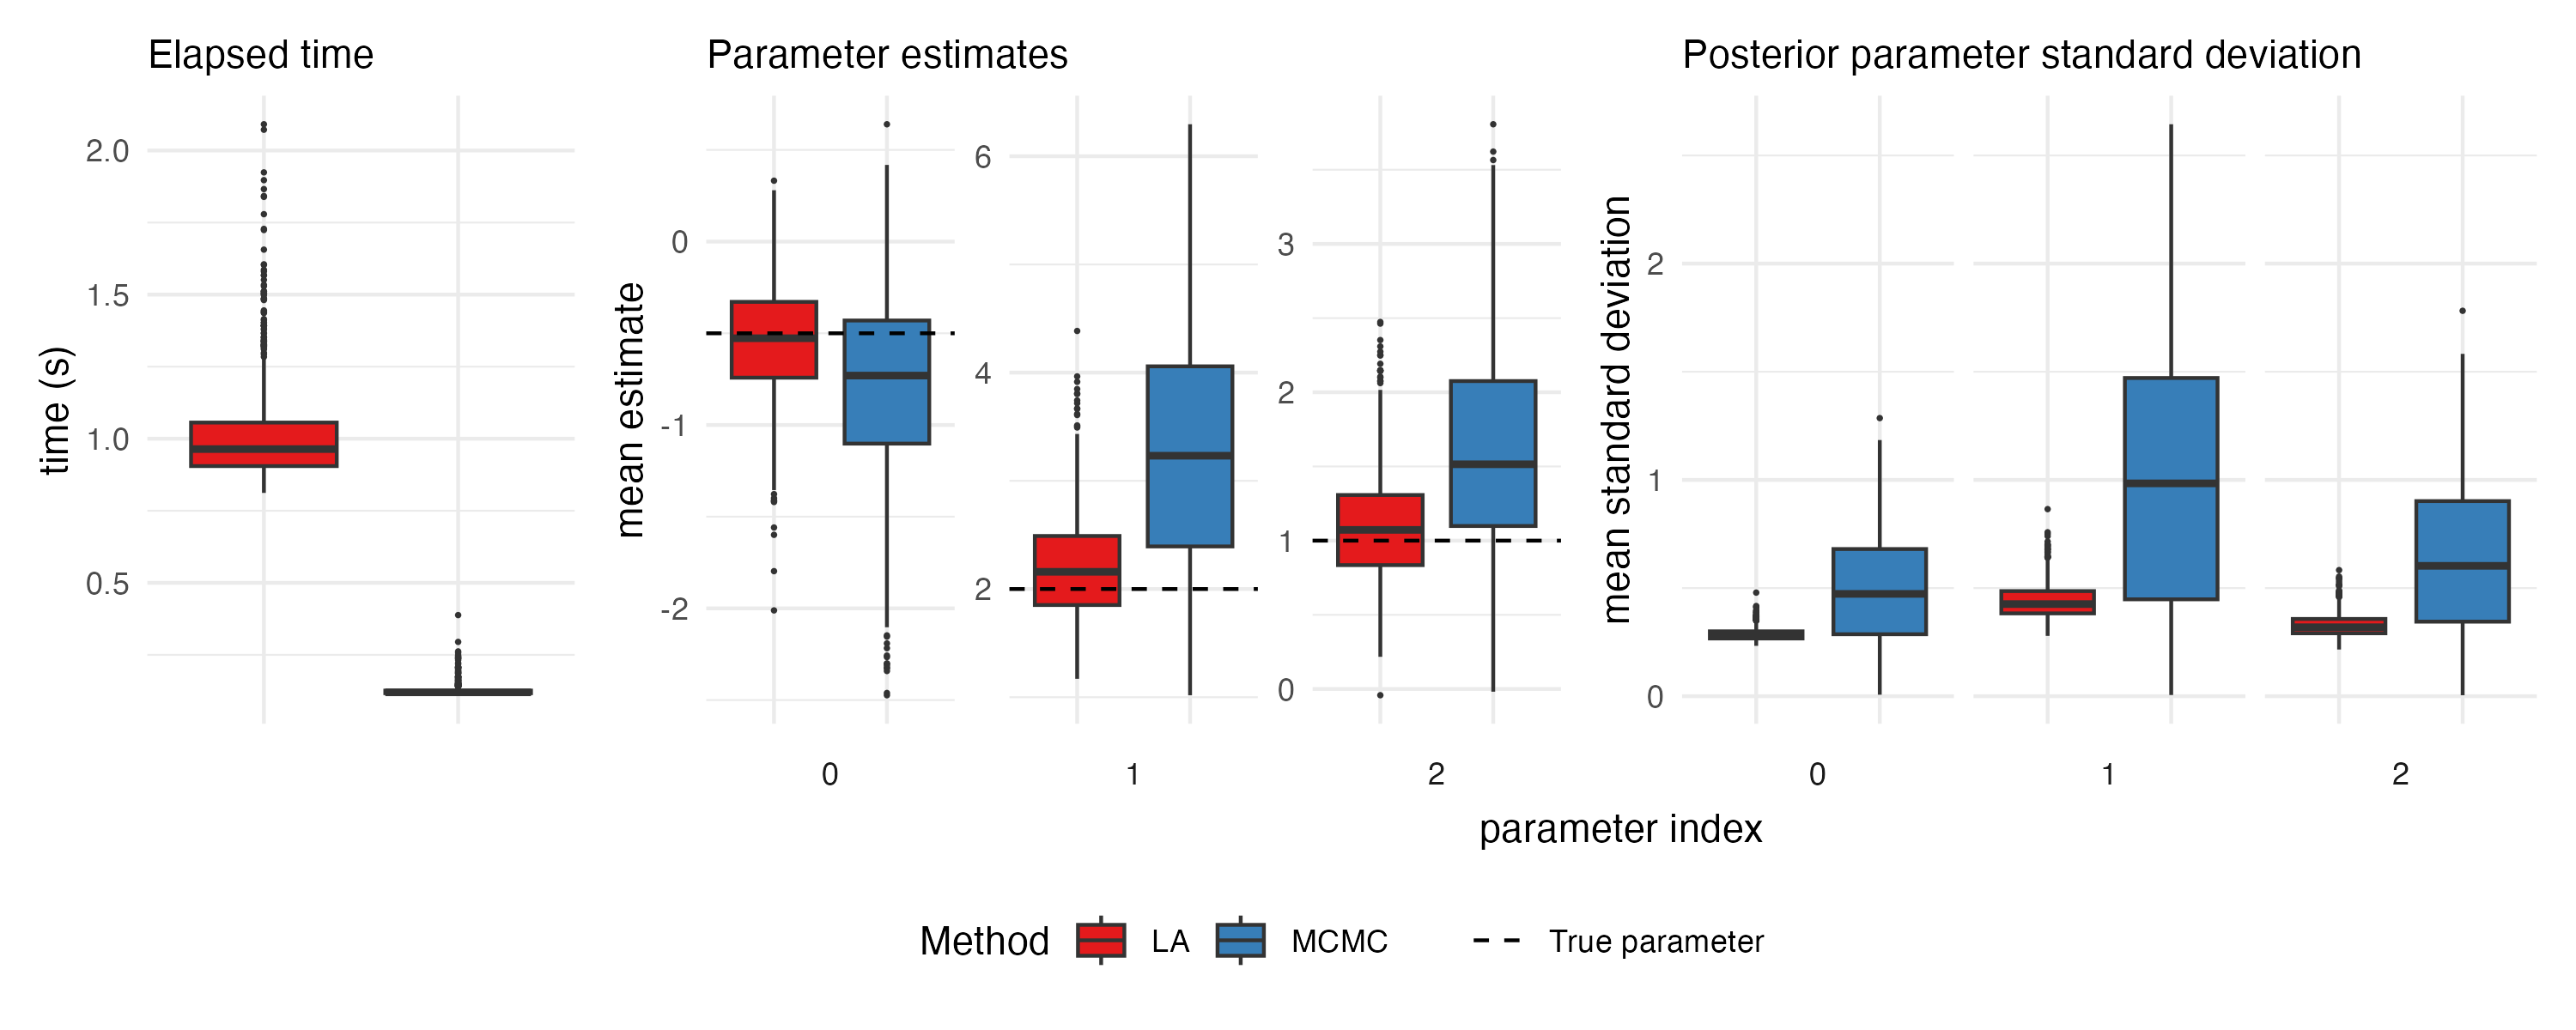
\includegraphics[width=\linewidth]{../figures/approx_class.png}
    \caption{
    Bayesian \textbf{logistic} regression: Comparison of LA (red) and MCMC (blue) across 1,000 simulations.
    LA outperforms MCMC in both accuracy and precision of parameter estimates.
    While LA is slower to compute, it provides more stable estimates.
    }
    \label{fig:approx-class}
\end{figure}

Results for the linear and logistic model can be seen in \autoref{fig:approx-regr} and \autoref{fig:approx-class} respectively.
In our experiment, inference with LA was generally slower than with MCMC methods.
There was not much difference in the posterior parameter estimates in the case of the Bayesian linear model (\autoref{fig:approx-regr}), although LA leads to a much higher standard deviation of parameters.
In contrast, LA showed clear advantages in logistic regression (\autoref{fig:approx-class}): it yielded more accurate parameter estimates and lower posterior uncertainty than MCMC.
These results highlight that the performance of approximate inference methods can differ significantly depending on the model and likelihood.


